\documentclass[a4paper]{article}
%AMDG
\usepackage{amsmath, amsthm, amssymb}
\usepackage{hyperref}
\usepackage[slovene]{babel}
\usepackage[utf8]{inputenc}
\usepackage[T1]{fontenc}
\usepackage{epigraph}
\usepackage{pdftexcmds}
\usepackage{fancyref, nameref}
\usepackage{epigraph}
\usepackage{cleveref}
\usepackage{verbatim}
\usepackage{enumitem}

\usepackage{tikz}


\parindent=0pt


% \epigraphsize{\small}% Default
\setlength\epigraphwidth{8cm}
\setlength\epigraphrule{0pt}

\usepackage{etoolbox}

\makeatletter
\patchcmd{\epigraph}{\@epitext{#1}}{\itshape\@epitext{#1}}{}{}
\makeatother


\newcounter{environment:definition_counter}

\newenvironment{definition}[1][\unskip]
{\vspace{0.5cm}\refstepcounter{environment:definition_counter}\textbf{Definicija \arabic{environment:definition_counter}: \textbf{#1}}\itshape}
{\bigskip}

\newcounter{environment:theorem_counter}

\newenvironment{theorem}[1][\unskip]
{\refstepcounter{environment:theorem_counter}\textbf{Izrek \arabic{environment:theorem_counter}:\textit{#1}} \\}
{\bigskip}

\newcounter{environment:statement_counter}

\newenvironment{statement}[1][\unskip]
{\refstepcounter{environment:statement_counter}\textbf{Trditev \arabic{environment:statement_counter}:\textit{#1}}}
{\bigskip}

\newcounter{example:example_counter}

\newenvironment{example}
{\textbf{Primer:}\\}
{\setcounter{example:example_counter}{0}}

\newenvironment{example_case}
{\refstepcounter{example:example_counter} \arabic{example:example_counter}.}
{\\}

\newenvironment{remark}
{\textbf{Opomba:}}
{}

\newenvironment{corollary}
{\underline{\textbf{Posledica:}}}
{}

%should rethink this
\newtheorem{lemma}{Lema}

\newcommand{\subscript}[2]{$#1 _ #2$}


\begin{document}
\title{Skripta za algebro 2}
\author{Filip Koprivec}
\date{\today}
\maketitle

\epigraph{“If I find in myself desires which nothing in this world can satisfy, the only logical explanation is that I was made for another world.”}{--- \textup{C. S. Lewis}}
\newpage

\tableofcontents

\newpage

\begin{comment}
Start of text
\end{comment}

\section{Osnovne algebrske strukture}
\subsection{Binarne operacije}
\begin{definition}[Binarna Operacija]
\label{def:binary_operation}
(tudi dvočlena operacija) $\circ$ na množici $\mathcal{S}$ je preslikava iz $\mathcal{S} \times \mathcal{S} \  v \ \mathcal{S}$.\\ Torej $\circ : \mathcal{S} \times \mathcal{S} \ \to \ \mathcal{S}$
\end{definition}

\begin{example}
Osnovna zgleda binarnih operacij na $\mathbb{Z}$ sta:

\begin{example_case}
Seštevanje: $(n,m) \mapsto n+m$
\end{example_case}
\begin{example_case}
Množenje: $(n,m) \mapsto n \times m$
\end{example_case}

\end{example}

Skalarni produkt v $\mathbb{R}^{2}$ \textbf{ni} binarna operacija.

Vektorski produkt v $\mathbb{R}^{3}$ \textbf{je} binarna operacija.
\\\\
\begin{definition}
\label{def:asociative_operation}
Operacija $\circ$ je \textbf{asociativna}, če ustreza enačbi
\begin{equation}
\label{eq:asociative_law}
\forall x,y,z \in \mathcal{S}.\ (x \circ y) \circ z = x \circ (y \circ z)
\end{equation}

\end{definition}

Enakost \ref{eq:asociative_law} imenujemo \textbf{Zakon o asociativnosti}\\
Operacije, ki jih bomo obravnavali bodo praviloma asociativne.

\begin{definition}
\label{def:comutative_operation}
Elementa $x,y \in \mathcal{S}$ \textbf{komutirata}, če velja 
\begin{equation}
x,y \in \mathcal{S}. x \circ y = y \circ x
\end{equation}
Če za poljubna dva elementa iz $\mathcal{S}$ velja
\begin{equation}
\label{eq:comutative_law}
\forall x,y \in \mathcal{S}. x \circ y = y \circ x
\end{equation}
pravimo, da je operacija $\circ$ komutativna.
Enakost \ref{eq:comutative_law} imenujemo \textbf{Zakon o komutativnosti}

\end{definition}
\begin{remark}
Kadar je iz konteksta razvidno, o kateri operaciji govorimo, pogosto namesto "$\circ$ je komutativna rečemo tudi $\mathcal{S}$ je komutativna"
\end{remark}

\begin{example}
\begin{example_case}
Operacija + na $\mathbb{Z}$ je tako asociativna in komutativna
\end{example_case}
\begin{example_case}
Operacija * na $\mathbb{Z}$ je tako asociativna in komutativna
\end{example_case}
\begin{example_case}
Operacija - na $\mathbb{Z}$ \textbf{ni} niti asociativna niti komutativna
\end{example_case}
\begin{remark}
Na operacijo odštevanja gledamo kot na izpeljano operacijo in ne kot na samostojna operacijo, saj jo vpeljemo preko seštevanja in pojma nasprotnega elementa.
\end{remark}

\begin{example_case}
Naj bo $\mathcal{X}$ poljubna neprazna množica. Z $F(\mathcal{X})$ označimo množico vseh preslikav iz $\mathcal{X}$ v $\mathcal{X}$. Naj bosta $f, g \in \mathcal{X}$, potem je $(f,g) \mapsto f \circ g$ (kompozitum funkcij) binarna operacija na $F(\mathcal{X})$.

\begin{remark}
Operacija je asociativna, in kadar $|\mathcal{X}| \geq 2$ ni komutativna
\end{remark}
\end{example_case}
\end{example}

\begin{definition}
\label{def:identity_element}
Naj bo $\circ$ binarna operacija na na $\mathcal{S}$ in $e \in \mathcal{S}$. $e$ se imenuje \textbf{nevtralni element}, če velja 
\begin{equation}
\label{eq:identity_element}
\forall x \in \mathcal{S}. e \circ x = x \circ e = x
\end{equation}

\end{definition}

\begin{example}
\begin{example_case}
$0$ je nevtralni element za seštevanje na $\mathbb{Z}$.
\end{example_case}
\begin{example_case}
$1$ je nevtralni element za množenje na $\mathbb{Z}$.
\end{example_case}
\begin{example_case}
$id_{x}$ (identična preslikava) je nevtralni element za $F(\mathcal{X})$
\end{example_case}
\end{example}

\begin{remark}
Nevtralni element nima zagotovljenega obstoja (recimo $+$ na $\mathbb{N}$ ali $*$ na sodih celih številih).
\end{remark}

\begin{statement}
\label{st:identity_unique}
Če nevtralni element obstaja, je en sam.
\begin{proof}
\label{pr:identity_unique}
Naj bosta $f,e \in \mathcal{S}$ nevtralna elementa.
$$e = e \circ f \text{\ \ // Ker je f nevtralni element}$$
$$e \circ f = f \text{\ \ // Ker je e nevtralni element}$$
$$e = f $$
\end{proof}
\end{statement}

\begin{definition}
\label{def:left_identity}
Element $e'$ je \textbf{levi nevtralni element}, če velja:
\begin{equation}
\label{eq:left_identity_element}
\forall x \in \mathcal{S}. e' \circ x = x
\end{equation}
\end{definition}

\begin{definition}
\label{def:right_identity}
Element $e''$ je \textbf{desni nevtralni element}, če velja:
\begin{equation}
\label{eq:right_identity_element}
\forall x \in \mathcal{S}. x \circ e'' = x
\end{equation}
\end{definition}

\begin{remark}
Levih in desnih nevtralnih elementov je lahko več

\begin{example}
\begin{example_case}
$\circ : (x,y) \mapsto y$.

Vsak element je levi nevtralni element
\end{example_case}
\begin{example_case}
$0$ je desni nevtralni element za odštevanje v $\mathbb{Z}$
\end{example_case}
\end{example}
\end{remark}

\begin{statement}
\label{st:identity_left_right_both}
Naj bo za operacijo $\circ$ $e'$ levi nevtralni element, $e''$ pa desni nevtralni element. Tedaj velja $e' = e'' = e$ (Sta si levi in desni nevtralni element enaka in je(sta) nevtralni element)
\begin{proof}
\label{pr:identity_left_right_both}
$$e' = e' \circ e'' = e''$$
\end{proof}
\end{statement}

\begin{definition}
\label{def:inner_operation}
Naj bo $\circ $ operacija na $\mathcal{S}$ in naj bo $\mathcal{T} \subseteq \mathcal{S}$. Rečemo, da je $\circ$ \textbf{notranja operacija na $\mathcal{T}$} ali da je množica \textbf{$\mathcal{T}$ zaprta za $\circ$ na $\mathcal{T}$} , če velja
\begin{equation}
\label{eq:inner_operation}
\forall t, t' \in \mathcal{T}. t \circ t' \in \mathcal{T}
\end{equation}

\end{definition}

\begin{example}
Množica $\mathbb{N}$ je zaprta za operaciji $+$ in $*$, ni pa zaprta za operacijo $-$.
\end{example}

\begin{definition}
\label{def:outer_operation}
Preslikavi iz $\mathcal{K} \times \mathcal{S}$ v $\mathcal{S}$ kjer $\mathcal{K} != \mathcal{S}$ rečemo \textbf{Zunanja binarna operacija}
\end{definition}

\begin{example}
\begin{example_case}
Množenje vektorja s skalarjem\\
$(\lambda, \vec{x}) \mapsto \lambda\vec{x}$, kjer je $(K = \mathbb{R}, S = \mathbb{R}^n)$\\
$\lambda (x_1, x_2, \dots , x_n) = (\lambda x_1, \lambda x_2, \dots ,\lambda x_n)$
\end{example_case}
\end{example}

\subsection{Polgrupe in monoidi}

\begin{definition}
\label{def:algebraic_structure}
\textbf{Algebrska struktura} je množica, opremljena z eno ali več operacijami (notranjimi ali zunanjimi), ki imajo določene lastnosti
\end{definition}

\begin{definition}
\label{def:semigroup}
\textbf{Polgrupa} je par množice $\mathcal{S}$ skupaj z \textbf{asociativno binarno operacijo}. Pišemo: $(\mathcal{S}, \circ)$
\end{definition}

\begin{remark}
Kadar je jasno o kateri operaciji govorimo, pogosto govorimo kar o polgrupi $\mathcal{S}$
\end{remark}

\begin{example}
\begin{example_case}
$(\mathbb{N}, +), \underbrace{(\mathbb{Z}, +), (\mathbb{Q}, +), (\mathbb{R}, +), (\mathbb{C}, +),\dots}_{Niso\ samo\ polgrupe\ ampak\ kar\ grupe}$
\end{example_case}
\end{example}
\\
\\
Naj bo $(\mathcal{S}, \circ)$ polgrupa, po zakonu \ref{eq:asociative_law} o asociativnosti velja:
$$\forall x,y,z \in \mathcal{S}.\ (x \circ y) \circ z = x \circ (y \circ z)$$zato lahko oklepaje spuščamo in vse to pišemo kot $x \circ y \circ z$. 
Kaj pa če imamo več kot tri elemente. Ali velja tudi:\\
$(x_1 \circ x_2) \circ (x_3 \circ x_4) = ((x_1 \circ x_2) \circ x_3) \circ x_4 = x_1 \circ (x_2 (\circ x_3 \circ x_4)) = \dots$

\begin{statement}
\label{def:semigroup_asociativity_operation}
Naj bo $(\mathcal{S}, \circ)$ polgrupa, $n \in \mathbb{N}$ in naj bo $x_1, x_2,\dots,x_n \in \mathcal{S}$. Tedaj je za vsak $n$ enakost izpolnjena na glede na postavitev oklepajev (izraz ima smisel, tudi kadar ne pišemo oklepajev).\\
$x_1 \circ x_2 \circ \dots \circ x_n = (\dots(x_1 \circ x_2) \circ \dots \circ x_n) = x_1 \circ (x_2 (\circ \dots \circ x_n)\dots) = \dots$
\end{statement}

\begin{proof}
\label{pr:semigroup_asociativity_operation}
Zgolj skica dokaza\\
Definirajmo:
$x:= x_1 \circ (x_2 (\circ \dots \circ x_n)\dots)$ in \\
$y:= $ naj bo kombinacija elementov $x_1 \dots x_n$, z drugače postavljenimi oklepaji\\
Indukcija na $n$:\\
$n \leq 3$: Očitno\\
Ker $n \leq 2$ velja $y = \underbrace{(u)}_{x_1, \dots, x_k} \circ \underbrace{(v)}_{x_{k+1}, \dots, x_n}$ Iz $k < n$ sledi:\\ $ y = (x_1 \circ w) \circ v \underbrace{=}_{Asociativnost (\ref{eq:asociative_law})} x_1 \circ ( w \circ v) $\\
Po I.P. ($w \circ v$ ima $n-1$ elementov):
$x = x_1 \circ (x_2 \circ \dots \circ x_{n})$
\end{proof}
Zato lahko oklepaje izpuščamo in pišemo kar:
$x_1 \circ x_2 \circ \dots \circ x_n$

\begin{definition}
\label{def:power_operation}
\textbf{Potenca elementa $x$.} Naj bo  $n \in \mathbb{N} - \{0\}$ in $x \in \mathcal{S}$
\begin{equation}
\label{eq:power_operation_natural}
x^n := \underbrace{x \circ x \circ \dots \circ x}_{n \text{elementov}}
\end{equation} 
\end{definition}

\begin{remark}
Brez asociativnosti ni definirano niti $x^3$
\end{remark}

\begin{remark}\\
Očitno velja:\\
$\forall n, m \in \mathbb{N}. x^n \circ x^m = x^{n+m}$ in \\
$\forall n, m \in \mathbb{N}. (x^n)^m = x^{n m}$
\end{remark}

\begin{definition}
\label{def:monoid}
\textbf{Polgrupa} z \textbf{nevtralnim elementom} se imenuje \textbf{monoid}.
\end{definition}
\begin{example}
\begin{example_case}
$(\mathbb{N}, +)$ \textbf{ni} monoid, $(\mathbb{N} \cup \{0\}, +)$ pa je.
\end{example_case}
\begin{example_case}
$(\mathbb{N}, *)$ je monoid
\end{example_case}
\begin{example_case}
$(F(\mathcal{X}), \circ)$ je monoid, nevtralni element je $id_{\mathcal{X}}$
\end{example_case}
\end{example}

\begin{definition}
\label{def:left_inverse}
Naj bo $( \mathcal{S}, \circ )$ monoid z nevtralnim elementom $e$. Element $y$ je \textbf{levi inverz}  elementa $x$, če velja: $y \circ x = e$.
\end{definition}

\begin{definition}
\label{def:right_inverse}
Naj bo $(\mathcal{S}, \circ)$ monoid z nevtralnim elementom $e$. Element $y$ je \textbf{desni inverz}  elementa $x$, če velja: $x \circ y = e$. 
\end{definition}

\begin{remark}
Levi in desni inverz nimata zagotovljenega obstoja, če pa obstajata ni nujno, da sta enolično določena.
\end{remark}

\begin{example}
\begin{example_case}
$f \in F(\mathcal{X})$ ima levi inverz $\iff f$ je injektivna\\
Če $f$ ni surjektivna ima lahko več levih inverzov, ki so izven $\mathcal{Z}_f$ lahko poljubno definirani.
\end{example_case}
\begin{example_case}
$f \in F(\mathcal{X})$ ima desni inverz $\iff f$ je surjektivna
\end{example_case}
\begin{example_case}
$f \in F(\mathcal{X})$ ima levi in desni inverz $\iff f$ je bijektivna
\end{example_case}
\end{example}

\begin{definition}
\label{def:inverse_element}
Element $y $ iz monoida $\mathcal{S}$ je inverz elementa $x$ Če velja:
\begin{equation}
x \circ y = y \circ x = e
\end{equation}
Elementu, ki ima inverz rečemo da je \textbf{obrnljiv} in njegov inverz označimo z $x^{-1}$(To ni čisto korektno, saj bomo šele malo naprej pokazali, da ima vsak element en sam inverz). In tako dobimo 
\begin{equation}
\label{eq:inverse_element}
x \circ x^{-1} = x^{-1} \circ x = e
\end{equation}
\end{definition}

\begin{remark}
Če je operacija $\circ$ komutativna potem levi inverz, desni inverz in inverz za posamezen element sovpadajo
\end{remark}
\\
\\
\begin{statement}
\label{st:inverse_left_right_both}
Naj bo $(\mathcal{S}, \circ)$ monoid, Če je $y$ levi inverz elementa $x$ in je $z$ njegov desni inverz, potem $z=y=x^{-1}$
\end{statement}
\begin{proof}
$y = y \circ e = y \circ (x \circ z) = (y \circ x) \circ z = e \circ z = z$
\end{proof}
\begin{corollary}
Obrnljiv element monoida ima natanko en inverz.
\end{corollary}

\begin{corollary}
Če je $x$ obrnljiv element monoida $\mathcal{S}$ potem iz $y \circ x = e$ sledi $x \circ y = e$.
\end{corollary}
\\
\begin{statement}
\label{st:pairwise_inverse}
Če sta $x$ in $y$ obrnljiva, potem je obrnljiv tudi element $(x \circ y)$ in je njegov inverz $y^{-1} \circ x^{_1}$
\end{statement}
\begin{proof}
\label{pr:pairwise_inverse}
To je desni inverz:\\
$(x \circ y)  \circ (y^{-1} \circ x^{-1}) = x \circ (y  \circ y^{-1}) \circ x^{-1} = x \circ e \circ x^{-1} = x \circ x^{-1} = e$\\
in tudi levi inverz:\\
$(y^{-1} \circ x^{-1}) \circ (x \circ y) = y^{-1} \circ (x^{-1} \circ x) \circ y = y^{-1} \circ e \circ y = y^{-1} \circ y = e$
\end{proof}
\begin{remark}
\label{rem:n_wise_inverse}
Seveda velja za $n$ elementov
\begin{equation}
\label{eq:n_wise_inverse}
(x_1 \circ  x_2 \circ \dots \circ x_n)^{-1} = x_{n}^{-1} \circ \dots \circ x_{2}^{-1} \circ x_{1}^{-1}
\end{equation}
\end{remark}

\begin{example}
\begin{example_case}
$(\mathbb{N} \cup \{0\}, +)$: edini obrnljiv element je 0.
\end{example_case}
\begin{example_case}
$(\mathbb{N}, *)$: edini obrnljiv element je 1
\end{example_case}
\begin{example_case}
$(\mathbb{Z}, *)$: edina obrnljiva elementa sta 1 in -1 
\end{example_case}
\begin{example_case}
$(\mathbb{Q}, *)$: Obrnljivi so vsi element razen 0
\end{example_case}
\begin{example_case}
$(F(\mathcal{X}), \circ)$: obrnljive so vse bijektivne preslikave
\end{example_case}
\end{example}
\begin{remark}
Poseben primer zadnje formule kadar je $x$ obrnljiv je tudi:$(x^n)^{-1} = (x^{-1})^n$ za $n \in \mathbb{N}$
\end{remark}

\begin{definition}
\label{def:integer_power}
\begin{equation}
\label{eq:integer_power}
n \in \mathbb{N}. x^{-n} := (x^n)^{-1} = (x^{-1})^n
\end{equation}
\end{definition}

\begin{definition}
\label{def:null_power}
\begin{equation}
\label{eq:null_power}
x^0 := e
\end{equation}

\end{definition}

Tako kadar je $x$ \textbf{obrnljiv} veljata enačbi

\begin{equation}
\label{eq:sum_of_powers}
\forall n, m \in \mathbb{Z}. x^n \circ x^m = x^{n+m}
\end{equation}

\begin{equation}
\label{eq:product_of_powers}
\forall n, m \in \mathbb{Z}. (x^n)^m = x^{n m}
\end{equation}

\begin{statement}
\label{st:reduction_rule}
Če je $x$ obrnljiv element monoida $\mathcal{S}$ potem velja \textbf{pravilo krajšanja}:
\begin{equation}
\label{eq:reduction_rule}
x \circ y = x \circ z \implies y = z
\end{equation}
In tudi
\begin{equation}
\label{eq:reduction_rule2}
y \circ x = z \circ x \implies y = z
\end{equation}
\begin{proof}
$$x \circ y = x \circ z \implies x^{-1} \circ x \circ y = x^{-1} \circ x \circ z \implies y = z$$
Druga enačba podobno
\end{proof}
\end{statement}

\begin{remark}
Iz enačbe $x \circ y = z \circ x$ v splošnem \textbf{ne} sledi $y = z$
\end{remark}

\subsection{Grupe}

\textbf{Dogovor:} V grupi bomo namesto $\circ$ uporabljali kar operacijo 'krat', torej se bo operacija imenovala kar množenje. Prav tako bomo izpuščali operator, ko bo le mogoče in pisali kar $xy$.

Tako $xy$ imenujemo 'produkt' $x$ in $y$, nevtralni element pa označimo z $1$ in mu rečemo kar \underline{enota}.

\begin{definition}
\label{def:group}
\textbf{Monoid} v katerem je \textbf{vsak element obrnljiv}, se imenuje \textbf{grupa}. Grupa, v kateri vsaka dva elementa komutirata, se imenuje \textbf{komutativna grupa} ali \textbf{Abelova grupa}.
\end{definition}

Ki je ekvivalenta bolj čisti definiciji:

\begin{definition}
\label{def:group_clean}
Množica $\mathbb{G}$ skupaj z binarno operacijo $* : \mathbb{G} \times \mathbb{G} \to \mathbb{G},\\ (x,y) \mapsto xy$ je \textbf{grupa} če zanjo velja:
\begin{enumerate}[label=\subscript{G}{\arabic*}:]
\item $$\forall x,y,z \in \mathbb{G}. \ (xy)z = x(yz)$$
\item $$\exists 1 \in \mathbb{G}. \ \forall x \in \mathbb{G}. \ 1x = x1 = x$$
\item $$\forall x \in \mathbb{G}. \ \exists x^{-1} \in \mathbb{G}. \  xx^{-1} = x^{-1}x = 1$$
\end{enumerate}
Če velja tudi:
$$\forall x,y \in \mathbb{G}. \ xy = yx$$
Potem grupo $\mathbb{G}$ imenujemo \textbf{Abelova} grupa.
\end{definition}



Grupe delim na komutativne in nekomutativne(glede na lastnosti operacije) ter na končne in neskončne(glede na število elementov).

\begin{example}
\begin{example_case}
$(\mathbb{Z}, +)$, $(\mathbb{Q}, +)$,$(\mathbb{R}, +)$,$(\mathbb{C}, +)$
\end{example_case}
\begin{example_case}
$(\mathbb{N} \cup \{0\}, +)$ \textbf{ni} grupa
\end{example_case}
\begin{example_case}
$(\mathbb{R}, *)$: \textbf{ni} grupa, ker 0 ni obrnljiv
\end{example_case}
\end{example}

\begin{remark}
Vsak monoid 'skriva' grupo.
\end{remark}

\begin{definition}
\label{def:monoid_invertible_elements}
S \textbf{$\mathcal{S}^*$} označujemo množico vseh obrnljivih elementov monoida $\mathcal{S}$.
\end{definition}

\begin{statement}
\label{st:subgroup_of_monoid}
Če je $\mathcal{S}$ monoid je $\mathcal{S}^*$ grupa.
\end{statement}

\begin{proof}
\label{pr:subgroup_of_monid}
$x, y \in \mathcal{S}^* \implies x \circ y \in \mathcal{S}^*$ // Obrnljiv je tudi njun produkt, torej je množica je zaprta za $*$ \\
Ker je $*$ asociativen na $\mathcal{S}$ je asociativen tudi na $\mathcal{S}^*$\\
$e \in \mathcal{S}^*$ saj je enota inverz sami sebi\\
$x \in \mathcal{S}^* \implies x^{-1} \in \mathcal{S}^*$ // Inverz inverza je kar element sam
\end{proof}

\begin{example}
\begin{example_case}
$(\mathbb{N} \cup \{0\}, +)$: $(\mathbb{N} \cup \{0\}, +)^* = {0}$
\end{example_case}
\begin{example_case}
$(\mathbb{Z}, +)$: $(\mathbb{Z}, +)^* = {-1,1}$ 
\end{example_case}
\begin{example_case}
$(\mathbb{Q}, *)$: $(\mathbb{Q}, *)^* = \mathbb{Q} - \{0\}$
\end{example_case}
\begin{remark}
Grupam z enim elementom pravimo \textbf{trivialne} grupe.
\end{remark}

\begin{example_case}
$(F(\mathcal{X}), \circ)$: $(F(\mathcal{X}), \circ)^* = \{f: \mathcal{X} \to \mathcal{X} | f \ \text{je bijekcija}\}$
\end{example_case}
\end{example}

\begin{definition}
\label{def:symetric_group}
Množico $Sim(\mathcal{X})$ imenujemo \textbf{simetrična grupa} (množice $\mathcal{X}$). 
\begin{equation}
\label{eq:general_symetric_group}
Sim(\mathcal{X}) := \{f: \mathcal{X} \to \mathcal{X} | f \ \text{je bijekcija}\}
\end{equation}
Njene elemente(bijektiven preslikave iz $\mathcal{X}$ v $\mathcal{X}$ pa imenujemo \textbf{permutacije} (množice $\mathcal{X}$).
\end{definition}

\begin{remark}
Če je množica končna jo praviloma označimo z $\{1,2,\dots, n\}$, njej pripadajočo grupo permutacij pa z
\begin{equation}
\label{eq:finite_symetric_group}
\mathcal{S}_n := Sim(\{1,2,\dots,n\})
\end{equation}
\end{remark}

Včasih bomo operacije na grupah vendarle označevali s $+$ ('seštevanje'). Taki grupi bomo rekli \textbf{aditivna grupa}. Nevtralni element bomo označevali z $0$, inverzni element pa bomo imenovali 'nasprotni element' in ga označevali z $-x$. Namesto $x+(-y)$ bom tako pisali $x-y$ (razlika $x$ in $y$). S tem smo v aditivno grupo vpeljali odštevanje. Prav tako bom namesto $x^n$ pisali $nx$. 

Primer takih grup so Abelove grupe. ($x+y = y+x$)

\subsection{Kolobarji}
$\mathbb{Z}, \mathbb{Q}, \mathbb{R}, \mathbb{C}$ so aditivne grupe, v katerih je naravno definirano tudi množenje, za katerega so monoidi.

\begin{definition}
\label{def:ring}
Množica $\mathcal{K}$ skupaj z binarnima operacijama seštevanja $+ : (x,y) \mapsto x+y$ in množenja $* : (x,y) \mapsto xy$ se imenuje \textbf{kolobar} če velja
\begin{enumerate}[label=\subscript{K}{\arabic*}:]
\item $(K, +)$ je \textbf{Abelova grupa}
\item $(K, *)$ je \textbf{monoid}
\item Izpolnjena sta oba distributivnostna zakona
\begin{equation}
\label{eq:left_distributive_law}
\forall x,y,z \in \mathcal{K}. \ z(x+y) = zx + zy
\end{equation}
\begin{equation}
\label{eq:right_distributive_law}
\forall x,y,z \in \mathcal{K}. \ (x+y)z = xz + yz
\end{equation}

\begin{remark}
Oba zakona potrebujemo zaradi ne nujne komutativnosti množenja v monoidu
\end{remark}
\end{enumerate}

\end{definition}

\begin{remark}
Poznamo tudi kolobarje brez enote (kjer je $(\mathcal{K}, *)$ zgolj monoid). Recimo $$2\mathbb{Z} := \{2n | n\in \mathbb{Z}\}$$
\end{remark}

\begin{statement}
V poljubnem kolobarju veljajo naslednje lastnosti:
\begin{enumerate}[label=(\alph*)]
\item 
$$\forall x \in \mathcal{K}. \ 0x = x0 = 0$$
\begin{proof}
$$0x = (0 + 0)x = 0x + 0x$$
$$\Downarrow$$
$$0 = 0x$$
Podobno za $x0=0$
\end{proof}
\item 
$$\forall x,y \in \mathcal{K}. \ (-x)y = x(-y) = -(xy)$$
\begin{proof}
$$0 = 0y = (x+(-y))y = xy + (-x)y$$
$$\Downarrow$$
$$-(xy) = (-x)y$$
\end{proof}
\item
$$\forall x,y,z \in \mathcal{K}. \ x(y-z) = xy -xz  \ \land \ (y-z)x = yx -zx$$
\begin{proof}
$$x(y-z) = x(y+(-z)) = xy + x(-z)$$
Podobno za drugo stran
\end{proof}
\item 
$$\forall x,y \in \mathcal{K}. \ (-x)(-y) = xy$$
\begin{proof}
$$(-x)(-y) = -(x(-y)) = -(-xy) = xy$$
\end{proof}
\item
$$\forall x \in \mathcal{K}. \ (-1)x = x(-1) = -x$$
Sledi iz (b) če vzamemo $y=-1$
\end{enumerate}
\end{statement}

Kolobar K je \textbf{komutativen}, če za množenje velja zakon komutativnosti (\ref{eq:comutative_law}).
\\

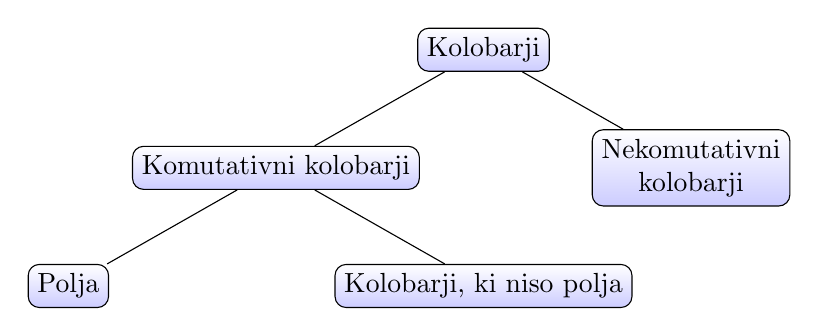
\begin{tikzpicture}[sibling distance=15em,
  every node/.style = {shape=rectangle, rounded corners,
    draw, align=center,
    top color=white, bottom color=blue!20}]]
  \node {Kolobarji}
    child { node {Komutativni kolobarji}
      child { node {Polja} }
      child { node {Kolobarji, ki niso polja} }
    }
    child { node {Nekomutativni \\ kolobarji} };
\end{tikzpicture}
\\
\\
\begin{example}
\begin{example_case}
$\mathbb{Z}$ (tipičen primer kolobarja)
\end{example_case}
\begin{example_case}
$\mathbb{Q}, \mathbb{R}, \mathbb{C}$ (to niso tipični primeri kolobarjev, saj so kar polja)
\end{example_case}
\begin{example_case}
\textbf{Trivialni} ali \textbf{ničelni kolobar}:
$$\{0\}$$
\end{example_case}
\begin{statement}
$$\text{Kolobar} \ \mathcal{K} \ \text{je ničelen} \iff 1=0$$

\begin{proof}\leavevmode \\
$\implies$: Očitno\\
$\impliedby$: $\forall x \in \mathcal{K}. \ x = 1x = 0x = 0$
\end{proof}
\end{statement}
\begin{example_case}
Matrični kolobarji ($M_{n}(\mathbb{R})$, $M_{n}(\mathbb{C})$) z običajnim seštevanjem in množenjem,
$$0 =
	\underbrace{\begin{bmatrix} 
		0 & 0 & \cdots & 0 \\
		0 & \ddots & \ddots & \vdots \\
		\vdots & \ddots & \ddots & 0 \\
		0 & \cdots & 0 & 0		
	\end{bmatrix}}_n; \ 
		1 =	\underbrace{\begin{bmatrix} 
		1 & 0 & \cdots & 0 \\
		0 & \ddots & \ddots & \vdots \\
		\vdots & \ddots & \ddots & 0 \\
		0 & \cdots & 0 & 1
	\end{bmatrix}}_n
$$
Ta kolobar je nekomutativen za $n \geq 2$\\
$ A = \begin{bmatrix}
		1 & 0 \\
		0 & 0
	  \end{bmatrix}
$;
$ B = \begin{bmatrix}
		0 & 1 \\
		0 & 0
	  \end{bmatrix}
$	
$\implies$
$AB = B, \ BA = 0$ \\
$A$ in $B$ ne komutirata, prav tako pa smo videlo da je lahko produkt dveh neničelnih elementov $0$.
\end{example_case}

\begin{definition}
\label{def:left_zero_divisor}
Element $x \neq 0$ kolobarja $\mathcal{K}$, je \textbf{levi delitelj niča}, če obstaja tak $y \neq 0, \in  \mathcal{K}$, da velja: $xy = 0$.
\end{definition}

\begin{definition}
\label{def:right_zero_divisor}
Element $x \neq 0$ kolobarja $\mathcal{K}$, je \textbf{desni delitelj niča}, če obstaja tak $y \neq 0, \in  \mathcal{K}$, da velja: $yx = 0$.
\end{definition}

\begin{definition}
Element $x$ je \textbf{delitelj niča}, če je \textbf{hkrati levi in desni delitelj niča}.
\end{definition}

\begin{remark}
\begin{equation}
\label{eq:left_zero_divisor_iff_right}
\mathcal{K} \ \text{ima leve deljitelje niča} \iff \mathcal{K} \  \text{ima deljitelje niča}
\end{equation}
\begin{proof}\leavevmode \\
$\implies$: Obstajata taka $y \neq 0, x \neq 0$, da je $xy = 0$. Imamo dve možnosti
\begin{enumerate}
\item $yx=0 \implies$ Dokaz je končan.
\item $yx \neq 0$: $x(yx) = 0 = (yx)y$ in je $yx$ desni delitelj niča .
\end{enumerate} 
$\impliedby$: Očitno.
\end{proof}
\end{remark}

V \textbf{Kolobarju brez deliteljev niča} velja:
\begin{equation}
\label{eq:xy_is_zero_implies_one_zero}
\forall x,y \in \mathcal{K}. \ xy = 0 \implies x = 0 \lor y = 0
\end{equation}

V takih kolobarjih velja pravilo krajšanja:
$$ xy = xz \land x  \neq 0 \implies y = z$$
$$ yx = zx \land x  \neq 0 \implies y = z$$
$$ xy = xz \iff x(y-z) = 0$$
$$ yx = zx \iff (y-z)x = 0$$
\end{example}

Kolobar je monoid za množenje zato lahko govorimo o obrnljivih elementih.
\begin{example}
\begin{example_case}
V $\mathbb{Z}$ sta obrnljiva $1, -1$.
\end{example_case}
\begin{example_case}
V $\mathbb{Q}, \mathbb{R}, \mathbb{C}$ so obrnljivi vsi elementi razen $0$
\end{example_case}
\end{example}

\begin{definition}
\label{def:skew_field}
Kolobar, v katerem $1 \neq 0$ in v katerem so \textbf{vsi neničelni elementi obrnljivi} se imenuje \textbf{obseg}.
\end{definition}

\begin{definition}
\label{def:field}
Komutativni obseg se imenuje \textbf{polje}
\end{definition}

\begin{example}
\begin{example_case}
$\mathbb{Q}, \mathbb{R}, \mathbb{C}$, so polja
\end{example_case}
\begin{example_case}
Nekomutativne obsege bomo dodali kasneje
\end{example_case}
\end{example}

\begin{statement}
\label{st:invertible_element_is_not_zero_divisor}
Obrnljiv element kolobarja ni levi(ali desni) delitelj niča.\\
Obsegi so zato kolobarji brez deliteljev niča.
\end{statement}
\begin{proof}
$x$ je obrnljiv: $xy=0$\\
$y = 1y = (x^{-1}x)y =  x^{-1}(xy) = x^{-1}0 = 0$ Torej $x$ ni delitelj niča.
\end{proof}

\subsection{Vektorski prostori}

\begin{definition}
\label{def:vector_space}
Naj bo $\mathcal{F}$ polje. Množica $\mathcal{V}$ skupaj z (notranjo) binarno operacijo seštevanje $+: \mathcal{V} \times \mathcal{V} \to \mathcal{V}$ in zunanjo binarno operacijo $\mathcal{F} \times \mathcal{V} \to \mathcal{V}$ imenovano \textbf{množenje s skalarji} in označeno z $(\lambda, v) \mapsto \lambda v$, se imenuje \textbf{vektorski prostor nad poljem $\mathcal{F}$}, če zanj velja:
\begin{enumerate}[label=\subscript{V}{\arabic*}:]
\item Za seštevanje je $\mathcal{V}$ Abelova grupa
\item Velja distributivnost v vektorskem faktorju
\begin{equation}
\label{eq:vector_space_vector_distributivity}
\forall \lambda \in \mathcal{F}. \  \forall u,v \in \mathcal{V}. \ \lambda(u+v) = \lambda u + \lambda v
\end{equation}
\item Velja distributivnost v skalarnem faktorju
\begin{equation}
\label{eq:vector_space_scalar_distributivity}
\forall \lambda, \mu \in \mathcal{F}. \  \forall v \in \mathcal{V}. \ (\lambda +\mu)v = \lambda v + \mu v
\end{equation}
\item Velja zakon homogenosti
\begin{equation}
\label{eq:vector_space_homogenous}
\forall \lambda, \mu \in \mathcal{F}. \  \forall v \in \mathcal{V}. \ (\lambda \mu)v = \lambda( \mu v)
\end{equation}
\item Enota
\begin{equation}
\label{eq:vector_space_unit}
 \forall v \in \mathcal{V}. \ 1v = v
\end{equation}
\end{enumerate}
\end{definition}

Za vsak vektorski prostor očitno veljajo naslednje trditve

\begin{itemize}
\item $$\forall \lambda \in \mathcal{F}. \ \lambda 0 = 0$$
\item $$\forall u,v \in \mathcal{V}. \  0x = 0$$
\item $$\forall \lambda, \mu \in \mathcal{F}. \  \lambda \mu = 0 \implies \lambda = 0 \lor \mu = 0$$
\item $$\forall \lambda, \mu \in \mathcal{F}. \ (-\lambda) \mu = \lambda(- \mu) = -(\lambda \mu) $$
\end{itemize}

\begin{remark}
Elementom polja $\mathcal{F}$ pravimo \textbf{skalarji}, elementom $\mathcal{V}$ pa vektorji
\end{remark}

\begin{itemize}
\item $\mathcal{F} = \mathbb{R}$: Realni vektorski prostor
\item $\mathcal{F} = \mathbb{C}$: Kompleksni vektorski prostor

\end{itemize}

\begin{example}
\begin{example_case}
Splošni prostor $\mathcal{F}^n$, kjer vpeljemo operaciji:\\
\textbf{Seštevanje}
\begin{equation}
\label{eq:vector_space_addition}
(u_1, u_2, \dots , u_n) + (v_1, v_2, \dots, v_n) \mapsto (u_1 + v_1, u_2 + v_2, \dots, u_n + v_n)
\end{equation}
\textbf{Množenje s skalarjem}
\begin{equation}
\label{eq:vector_space_scalar_multiplication}
\lambda (u_1, u_2, \dots , u_n) \mapsto (\lambda u_1 , \lambda u_2 , \dots, \lambda u_n)
\end{equation}
\end{example_case}
\begin{example_case}
Trivialni vektorski prostor: $\{0\}$
\end{example_case}
\begin{example_case}
Vektorski prostor polinomov stopnje največ $n$, kjer seštevanje in množenje definiramo na običajen način
\end{example_case}
\begin{example_case}
$\mathbb{C}$ je vektorski prostor nad $\mathbb{R}$ ( za $+$ je Abelova grupa, množenje pa definiramo po komponentah, tako je nad $\mathbb{R}$ to $2$-dimenzionalen, nad $\mathbb{C}$ pa $1$-dimenzionalen)
\end{example_case}
\end{example}

\subsection{Algebre}
Mnogi pomembni primeri kolobarjev so hkrati tudi vektorski prostori, dejansko so algebre.

\begin{definition}
\label{def:algebra}
Naj bo $\mathcal{F}$ polje (komutativen obseg). Množica $\mathcal{A}$ skupaj z (notranjima) binarnima operacijama $+$ (seštevanje) in $*$ (množenje) ter zunanjo binarno operacijo $\mathcal{F} \times \mathcal{A} \to \mathcal{A}$ (množenje s skalarji) je \textbf{Algebra na poljem $\mathcal{F}$ ali $\mathcal{F}$-algebra}, če velja:
\begin{enumerate}[label=\subscript{V}{\arabic*}:]
\item Za seštevanje in množenje s skalarji je $\mathcal{A}$ vektorski prostor
\item Za množenje je $\mathcal{A}$ monoid
\item Veljata neke vrste levi in desni distributivnostni zakon
$$\forall x,y,z \in \mathcal{A}. \ \forall \lambda, \mu \in \mathcal{F}. \ (\lambda x + \mu y) z = \lambda(xz) + \mu(yz)$$
$$\forall x,y,z \in \mathcal{A}. \ \forall \lambda, \mu \in \mathcal{F}. \ z(\lambda x + \mu y) = \lambda(zx) + \mu(zy)$$

\begin{remark}
Za $\lambda = \mu = 1$ je to navadna distributivnost. Torej je algebra kolobar, ki je hkrati vektorski prostor, v katerem velja še:
$$\lambda(xz) = (\lambda x)z = x(\lambda z)$$
\end{remark}

\end{enumerate}

\end{definition}


\begin{example}
\begin{example_case}
Vektorski prostor $\mathcal{F}^n$ postane algebra, če definiramo množenje, najlažje kar po komponentah:
\begin{equation}
\label{eq:vector_space_to_algebra_component_mulitplication}
(x_1, x_2, \dots, x_n) (y_1, y_2, \dots, y_n) \mapsto (x_1 y_1,, x_2 y_2, \dots, x_n y_n)
\end{equation} 
\end{example_case}
\begin{example_case}
Kolobar $M_n(\mathbb{R})$ postane algebra, če definiramo množenje s skalarji
\begin{equation}
\label{eq:matrix_scalar_multiplication}
\lambda (a_{ij}) = (\lambda a_{ij})
\end{equation}
\end{example_case}
\begin{example_case}
Vektorski prostor polinomov postane algebra, če vpeljemo množenje polinomov na standardni način
\end{example_case}
\end{example}

\begin{remark}
'Teorija kolobarjev' in 'teorija kolobarjev in algeber' se razlikujeta zgolj v poudarku.
\end{remark}

\subsection{Podgrupe, podkolobarji in druge podstrukture}
$(\mathbb{R}, +)$ in $(\mathbb{C}, +)$ sta različni strukturi, a očitno povezani Abelovi grupi. Operacija je seštevanje in $\mathbb{R} \subseteq \mathbb{C}$. Rečemo: $(\mathbb{R}, +)$ je podgrupa $(\mathbb{C}, +)$. \\
Podobno rečemo 
$(\mathbb{R}, +, *)$ je podkolobar $(\mathbb{C}, +, *)$\\
In ker sta to tudi polji rečemo kar kar $(\mathbb{R}, +, *)$ je podpolje $(\mathbb{C}, +, *)$\\

\subsubsection{Podgrupe}
\begin{definition}
\label{def:subgroup}
\textbf{Neprazna} podmnožica $\mathcal{H}$ grupe $\mathcal{G}$ je \textbf{podgrupa} grupe $\mathcal{G}$, če je za isto operacijo (zožitev na $\mathcal{H} \times \mathcal{H}$) tudi sama grupa. 
\end{definition}

\begin{example}
\begin{example_case}
Vsaka grupa $\mathcal{G}$ ima vsaj dve podgrupi: $\mathcal{G}$ in $\{1\}$\\
\begin{remark}
$\{1\}$ se imenuje \textbf{trivialna podgrupa}
\end{remark}

\begin{remark}
Vsaka od $\mathcal{G}$ različna podgrupa se imenuje \textbf{prava podgrupa}
\end{remark}
\end{example_case}

\end{example}

\begin{statement}
\label{st:subgroup_equivalent_defintions}
Za neprazno podmnožico $\mathcal{H}$ grupe $\mathcal{G}$ so naslednje trditve ekvivalentne:
\begin{enumerate}[label=(\roman*)]
\item $$\mathcal{H} \ \text{je podgrupa} \ \mathcal{G}$$
\item $$\forall x,y \in \mathcal{H}. \ x y^{-1} \in \mathcal{H}$$ 
\item $$\forall x,y \in \mathcal{H}. \ x y \in \mathcal{H} \land x^{-1} \in \mathcal{H}$$ 
\end{enumerate}
\end{statement}
\begin{proof}
\label{pr:subgroup_equivalent_defintions}\leavevmode \\
(i) $\implies$ (ii) : Očitno iz definicije da je $\mathcal{H}$ grupa \\
(ii) $\implies$ (iii) : \\
$$x \in \mathcal{H} \Longrightarrow 1 = x x^{-1} \in \mathcal{H} \Longrightarrow x^{-1} = 1 x^{-1} \in \mathcal{H} \ \text{// Zaprta za inverz}$$
$$x,y \in \mathcal{H} \Longrightarrow x y = x (y^{-1})^{-1} \in \mathcal{H} \ \text{Zaprta za poljubna dva}$$
(iii) $\implies$ (i):\\
Očitno zaprta za množenje, asociativna, ker velja na večji množici ($\mathcal{G}$)
$$1 = x x^{-1} \in \mathcal{H}$$
$$x \in \mathcal{H} \implies x^{-1} \in \mathcal{H}$$
\end{proof}

Govorimo 'grupa $\mathcal{H}$' ali 'podgrupa $\mathcal{H}$' označimo:

$$\mathcal{H} \leq \mathcal{G}$$

\begin{example}
\begin{example_case}
$\mathbb{R} - \{0\}$ je podgrupa $(\mathbb{C}-\{0\})$
\end{example_case}
\begin{example_case}
$\{x \in \mathbb{R} | x < 0\}$ je podgrupa $(\mathbb{C}-\{0\})$
\end{example_case}
\begin{example_case}
$\{1, -1, i, -i\}$ je podgrupa $(\mathbb{C}-\{0\})$
\end{example_case}
\begin{example_case}
$\{z \in \mathbb{C} | \ |z| = 1\}$ je podgrupa $(\mathbb{C}-\{0\})$
\end{example_case}
\begin{example_case}
$\{x \in \mathbb{R} | \ |x| > 1\}$ \textbf{ni} podgrupa $(\mathbb{C}-\{0\})$
\end{example_case}
\begin{example_case}
$\{z \in \mathbb{C} - \{0\} | \ |z| \leq 1\}$ \textbf{ni} podgrupa $(\mathbb{C}-\{0\})$
\end{example_case}
\end{example}

\begin{remark}\\
V aditivni grupi velja \\(ii) :  $\forall x,y \in \mathcal{H}. \ x - y \in \mathcal{H}$ in \\
(iii): $\forall x,y \in \mathcal{H}. \ x + y \in \mathcal{H} \land -x \in \mathcal{H}$
\end{remark}
\\

\begin{example}
Podgrupe $(\mathbb{Z}, +)$\\
\begin{example_case}
Trivialna primera podgrup sta $\mathbb{Z}$ in $\{0\}$
\end{example_case}
\begin{example_case}
$2\mathbb{Z} = \{2n | n \in \mathbb{Z}\}$
\end{example_case}
\begin{example_case}
$k\mathbb{Z} = \{kn | n \in \mathbb{Z}\}$ // $k \in \mathbb{Z}$
\end{example_case}
\end{example}

\begin{definition}
\label{def:conjugate_elements_group}
Elementa $a, b$ iz grupe $\mathcal{G}$ sta si \textbf{konjugirana}, če velja:
\begin{equation}
\label{eq:conjugate_element_group}
\exists c \in \mathcal{G}. \ b = c a c^{-1}
\end{equation}
\begin{remark}
Relacija 'elementa sta si konjugirana' je ekvivalenčna.
\end{remark}
\end{definition}

\begin{statement}
\label{def:conjugate_subgroup}
Če je $c \in \mathcal{H} \leq \mathcal{G}$, je 
\begin{equation}
\label{eq:conjugate_subgroup}
c \mathcal{H} c^{-1} := \{ chc^{-1} | \ h \in \mathcal{H}\}
\end{equation}
\textbf{konjugirana podgrupa} podgrupe $\mathcal{H}$.
\end{statement}

\begin{proof}
\label{st:conjugate_subgroup_is_subgroup}
$$chc^{-1} c h' c^{-1} = c\underbrace{hh'}_{\in \mathcal{H}}c^{-1} \in \mathcal{H}$$
$$(chc^{-1})^{-1}  = (c^{-1})^{-1}h^{-1}c^{-1} = c \underbrace{h^{-1}}_{ \in \mathcal{H}} c^{-1} \in \mathcal{H}$$
\end{proof}

\begin{remark}
Pojem konjugiranih podgrup ima smisel v nekomutativnih grupah
\end{remark}

\subsubsection{Podkolobarji}

\begin{definition}
\label{def:sub_ring}
Podmnožica $\mathcal{L}$ kolobarja $\mathcal{K}$ je \textbf{podkolobar} kolobarja $\mathcal{K}$, če vsebuje enoto \{1\} kolobarja $\mathcal{K}$ in če je kolobar za isti operaciji. 
\end{definition}

\begin{example}
\begin{example_case}
$\mathcal{L} = \{ \begin{bmatrix}
		x & 0 \\
		0 & 0
	  \end{bmatrix} | \ x \in \mathbb{R}\}$\\
	  Sicer je kolobar za isti operaciji, a ne podeduje enote (ima svojo), torej \textbf{ni} podkolobar.
\end{example_case}
\end{example}

\begin{statement}
\label{st:sub_ring_closed_for_inverse}
Podmnožica $\mathcal{L}$ kolobarja $\mathcal{K}$ je podkolobar natanko tedaj, ko velja
\begin{equation}
\label{eq:sub_ring_closed_for_inverse}
1 \in \mathcal{L} \land 
\forall x, y \in \mathcal{L}. \ x-y \in \mathcal{L}
\end{equation}
\end{statement}

\begin{proof}\leavevmode \\
\label{pr:sub_ring_closed_for_inverse}
$\implies$: Sledi iz definicije\\
$\impliedby$ Iz predpostavke sledi, da je $\mathcal{L}$ podgrupa za $+$.\\ Prav tako je $(\mathcal{L}, *)$ monoid\\ Izpolnjevanje distributivnih zakonov pa sledi iz tega da so izpolnjeni tudi na $\mathcal{K}$
\begin{remark}
Uporabili smo trditev (\ref{st:subgroup_equivalent_defintions}) in (ii) pogoj zamenjali z (iii)
\end{remark}
\end{proof}

\begin{example}
\begin{example_case}
Kolobar $\mathbb{Z}$ je podkolobar $\mathbb{Q}$.
\end{example_case}
\begin{example_case}
Kolobar $\mathbb{Q}$ je podkolobar $\mathbb{R}$.
\end{example_case}
\end{example}

\subsubsection{Podprostori}
\begin{definition}
\label{def:vector_subspace}
Podmnožica $\mathcal{U}$ vektorskega prostora $\mathcal{V}$ je \textbf{podprostor} $\mathcal{V}$, če je za isti operaciji tudi sama vektorski prostor.
\end{definition}

\begin{statement}
Za neprazno podmnožico $\mathcal{U}$ vektorskega prostora $\mathcal{V}$ so naslednje trditve ekvivalentne
\begin{enumerate}[label=(\roman*)]
\item $$\mathcal{U} \ \text{je podprostor} \ \mathcal{V}$$
\item $$\forall x, y \in \mathcal{U}. \ \forall \lambda, \mu \in \mathcal{F}. \ \lambda x + \mu y \in \mathcal{U}$$
\item $$\forall x, y, \in \mathcal{U}. \  x + y \in \mathcal{U} \land \forall x \in \mathcal{U}. \  \forall \lambda \in \mathcal{F}. \ \lambda x  \in \mathcal{U}$$
\end{enumerate}	
\end{statement}

\begin{proof}
Očitno
\end{proof}

\begin{example}
Edini podprostori vektorskega prostora $\mathbb{R}^3$ so:
\begin{itemize}
\item $\{0\}$, $\mathbb{R}^3$
\item premice skozi izhodišče
\item ravnine skozi izhodišče
\end{itemize}
\end{example}

\subsubsection{Podalgebre}
\begin{definition}
\label{def:subalgebra}
Podmnožica $\mathcal{B}$ algebre $\mathcal{A}$ je \textbf{podalgebra} $\mathcal{A}$, če je za iste operacije tudi sama algebra in vsebuje enoto \{1\} iz algebre $\mathcal{A}$.
\end{definition}

\begin{statement}
Neprazna podmnožica $\mathcal{B}$ algebre $\mathcal{A}$ je \textbf{podalgebra} algebre $\mathcal{A}$ natanko tedaj ko zanjo velja:
\begin{equation}
\label{eq:is_subalgebra}
1 \in \mathcal{B} \land \forall x, y \in \mathcal{B}. \ \forall \lambda \in \mathcal{F}. \ \underbrace{x+y, \lambda x}_{podprostor}, xy \in \mathcal{B}
\end{equation}
Torej je zaprta za seštevanje, množenje in množenje s skalarji
\end{statement}

\begin{proof}
Enako kot za podkolobarje
\end{proof}

\begin{example}
\begin{example_case}
$A = \mathcal{M}_2(\mathbb{R})$, 
$B = \{ \begin{bmatrix}
		a_{11} & a_{12} \\
		0 	   & a_{22}
	  \end{bmatrix} | a_{ij} \in \mathbb{R} \}$
\leavevmode
\end{example_case}
\end{example}

\subsubsection{Podpolje}

\begin{definition}
\label{def_subfield}
Podmnožica $\mathcal{F}$ polja $\mathcal{E}$ je \textbf{podpolje} polja $\mathcal{E}$, če je za isti operaciji tudi sama polje
\end{definition}

\begin{remark}
Podpolje nujno vsebuje isto enoto $1$ kot polje $\mathcal{E}$, naj bo $e \in \mathcal{F}$ enota.
$e^2 = e \implies e(\underbrace{1}_{enota \ \mathcal{E}}- \ e) = 0$ Ker v poljih ni deliteljev niča, velja $e=1$.
\end{remark}

\begin{statement}
Podmnožica $\mathcal{F} \neq \{0\}$ polja $\mathcal{E}$ je podpolje natanko tedaj ko velja
\begin{equation}
\label{eq:subfield_equivalent_definition}
\forall x, y \in \mathcal{F}. \ xy, x-y \in \mathcal{F} \land 0 \neq x \in \mathcal{F}. \ x^{-1} \in \mathcal{F} 
\end{equation}
\end{statement}

\begin{proof}Podobno kot prej
	
\end{proof}

\begin{statement}
$\mathcal{F} = \{0\} \iff 1 = 0$
\begin{proof}\leavevmode\\
$\implies$

$\forall x \in \mathcal{F}. \ 0x = x$ torej je $0$ nevtralni element

$\impliedby$

$\forall x \in \mathcal{F}. \ x = 1x = 0x = 0$ vsi elementi so ničelni
\end{proof} 
\end{statement}


\begin{definition}
\label{def:field_extension}
Polje $\mathcal{E}$ je \textbf{razširitev} polja $\mathcal{F}$ če je $\mathcal{F}$ podpolje $\mathcal{E}$.
\end{definition}

\begin{example}
\begin{example_case}
$\mathbb{R}$ je podpolje $\mathbb{C}$
\end{example_case}
\begin{example_case}
$\mathbb{C}$ je razširitev $\mathbb{R}$, ki je razširitev $\mathbb{Q}$
\end{example_case}
\end{example}


\subsubsection{Logične operacije nad (pod)strukturami}
Če so $\mathcal{H}_i$ podgrupe grupe $\mathcal{G}$ je tudi njihov presek $\cap \mathcal{H}_i$ podgrupa.

\begin{remark}
Družina $\mathcal{H}_i$ je \textbf{lahko končna ali neskončna} torej poljubna
\end{remark}\\

\textbf{Presek} algebrskih struktur (podgrup, podkolobarjev, podprostorov, podalgeber, podpolji) \textbf{ohrani lastnosti} te algebrske strukture.\\

\textbf{Unija} algebrskih struktur praviloma \textbf{ne ohrani} lastnosti te algebrske strukture.

\begin{example}
\begin{example_case}
$2\mathbb{Z} = \{2n | n \in \mathbb{Z}\}$ in $3\mathbb{Z} = \{3n | n \in \mathbb{Z}\}$ sta podgrupi $\mathbb{Z}$, njuna unija pa ni podgrupa (saj ni grupa), ker $2+3=5 \notin 2\mathbb{Z} \cup 3\mathbb{Z}$
\end{example_case}
\end{example}

\subsection{Generatorji}
$\mathbb{R}^3$ je generiran z vektorji: $(1,0,0), (0,1,0), (0,0,1)$. Edini podprostor, ki te vektorje vsebuje je namreč $\mathbb{R}^3$ sam. Seveda je generiran tudi z drugimi vektorji: $(1,1,0), (0,1,0), (0,0,1)$.\\
Vektorja $(1,0,0),(0,1,0)$ pa generirata ravnino: $z=0$.

\subsubsection{Generatorji grup}
Naj bo $\mathcal{X}$ neprazna podmnožica grupe $\mathcal{G}$, Vzemimo množico vseh elementov oblike $x_1 x_2 \dots x_n$, kjer velja $x, x^{-1} \in \mathcal{X}$ in jo označimo z $<\mathcal{X}>$.
 
Če je $\mathcal{X} = \{y_1, y_2, \dots , y_n\}$ pišemo tudi $\mathcal{X} = <y_1, y_2, \dots , y_n>$. 

Tako $<x,y>$ sestoji iz elementov kot so: $1, x, y, x^2, x^3, x^{-1}, x^{-2}, x^{-1}y, y^{-1}, x^5y^{-1}x^3y^{-3}xy^2, \dots$
\textbf{Opazimo}, da je $<\mathcal{X}>$ podgrupa
$$u,v \in <x> \implies uv \in <\mathcal{X}> \land u^{-1} \in <x>$$
$(x_1,\dots, x_n)^{-1} = x_{1}^{-1} \dots x_n^{-1}$, ki vsebuje množico $\mathcal{X}$.

Velja pa tudi obratno: vsaka podgrupa grupe $\mathcal{G}$, ki vsebuje $\mathcal{X}$ vsebuje tudi to podgrupo($<\mathcal{X}>$).

Torej je $<\mathcal{X}>$ najmanjša podgrupa, ki vsebuje $\mathcal{X}$. Pravimo ji \textbf{podgrupa, generirana z $\mathcal{X}$}.

Če velja $<\mathcal{X}> = \mathcal{G}$, rečemo, da je $\mathcal{G}$ generirana z množico $\mathcal{X}$, elemente iz $\mathcal{X}$ pa imenujemo \textbf{generatorji} grupe $\mathcal{G}$, množici $\mathcal{X}$ pa \textbf{množica generatorjev}.\\

\begin{example}
\begin{example_case}
$\mathbb{Q}^+$ je grupa za množenje. Velja: $<\mathbb{N}> = \mathbb{Q}^+$
\end{example_case}
\begin{example_case}
$<2,3> = \{2^i 3^j | i,j \in \mathbb{Z}\}$
\end{example_case}
\end{example}

\begin{remark}
V aditivni grupi $<\mathcal{X}>$ za komponiranje elementov uporabljamo drugo operacijo, vse ostalo ostane isto.
\end{remark}\\

\begin{example}
\begin{example_case}
Grupa $(\mathbb{Z}, +)$ je generirana z $<1>$ in prav tako tudi z $<-1>$. Velja $\mathbb{Z} = <1> = <-1>$.
\end{example_case}
\end{example}

\begin{remark}
Grupe generirane z enim samim elementom imenujemo \textbf{ciklične}.($<2> = <4,6> = 2\mathbb{Z}$)

\end{remark}

Cilj je poiskati najmanjše množice generatorjev(očitno $<\mathcal{G}> = \mathcal{G}$).

\begin{definition}
\label{def:finitly_generated_group}
Grupa je \textbf{končno generirana} če je generirana s kako končno množico.
\end{definition}

\subsubsection{Generatorji kolobarja}
Naj bo $\mathcal{K}$ kolobar, $\emptyset \neq \mathcal{X} \subseteq \mathcal{K}$.

Označimo z $\overline{\mathcal{X}}$ podgrupo za seštevanje $\mathcal{K}$, ki vsebuje vse produkte elementov iz $\mathcal{X} \cup \{1\}$.

Opazimo: $\overline{\mathcal{X}}$ je podkolobar, ki vsebuje $\mathcal{X}$ in je vsebovan v vsakem podkolobarju, ki $\mathcal{X}$ vsebuje. Zato mu rečemo \textbf{podkolobar generiran z množico $\mathcal{X}$}.

\begin{example}
\begin{example_case}
$\mathcal{K} = \mathbb{C}$
\begin{itemize}
\item $\overline{\{1\}} = \mathbb{Z}$
\item $\overline{\{i\}} = \{ n + mi | n,m \in \mathbb{Z}\} = \mathbb{Z}[i]$ (Kolobar \textbf{Gaussovih celih števil})
\end{itemize}\leavevmode
\end{example_case}
\end{example}

\begin{remark}
Pojme, kot so \textbf{generator kolobarja, končno generiran kolobar,\dots} definiramo enako kot za grupo.
\end{remark}

\subsubsection{Generatorji vektorskih prostorov}

\begin{definition}
\label{def:linear_combination}
Naj bo $\mathcal{V}$ vektorski prostor nad $\mathcal{F}$. Vsakemu vektorju $v$ oblike
\begin{equation}
\label{eq:linear_combination}
v = \lambda_1 v_1 + \dots + \lambda_n v_n; \lambda_i \in \mathcal{F} \land v_i \in \mathcal{V}
\end{equation}
pravimo \textbf{linearna kombinacija} vektorjev $v_1, v_2, \dots, v_n$.
\end{definition}


\begin{definition}
\label{def:linear_spang_enerated}Naj bo 
$\emptyset \neq \mathcal{X} \subseteq \mathcal{V}$. Podprostor generiran z $\mathcal{X}$, torej podprostor, ki $\mathcal{X}$ vsebuje in je vsebovan v vsakem podprostoru, ki vsebuje $\mathcal{X}$, je množica $\mathcal{L}(\mathcal{X})$, vseh linearnih kombinacij vektorjev iz $\mathcal{X}$, $\mathcal{L}(\mathcal{X})$ imenujemo \textbf{linearna lupina množice $\mathcal{X}$}.
\end{definition}


\begin{definition}
Naj bo $\mathcal{X}$ množica generatorjev za $\mathcal{V}$, tedaj $\mathcal{X}$ imenujemo \textbf{ogrodje $\mathcal{V}$}. Velja še $\mathcal{L}(\mathcal{X}) = \mathcal{V}$.
\end{definition}

\begin{remark}
Posebnost vektorskega prostora je v tem, da imamo pojem \textbf{linearne neodvisnosti}, preko katerega vpeljemo pojem \textbf{baze} vektorskega prostora.
\end{remark}


\subsubsection{Generatorji algeber}

\begin{definition}
\label{def:subalgebra_generated}
Naj bo $\mathcal{A}$ algebra na $\mathcal{F}$, naj bo $\emptyset \neq \mathcal{X} \subseteq \mathcal{A}$. \textbf{Podalgebra generirana z $\mathcal{X}$} je množica, ki sestoji iz elementov $x$ oblike
\begin{equation}
\label{eq:subalgebra_generated_element}
x = \lambda_1 x_{11} x_{12} \dots x_{1n_1} + \dots + \lambda_r x_{r1} x_{rn_r}; \lambda_i \in \mathcal{F} \land x_i \in \mathcal{X} \cup \{1\}
\end{equation}
\end{definition}



\begin{example}
\begin{example_case}
$\mathcal{A} = \mathcal{M}_2(\mathbb{R})$ 
\begin{itemize}
\item Podalgebra generirana z:

$e_{11} = \begin{bmatrix}
		1 & 0 \\
		0 & 0
	  \end{bmatrix}$, 
$e_{22} = \begin{bmatrix}
		0 & 0 \\
		0 & 1
	  \end{bmatrix}$
	  
je algebra diagonalnih matrik: 
$$\begin{bmatrix}
	   \lambda & 0 \\
		0 & \mu
		
	  \end{bmatrix}; \ \lambda, \mu \in \mathbb{R}$$ 
\item Podalgebra generirana z:

$e_{11} = \begin{bmatrix}
		0 & 1 \\
		0 & 0
	  \end{bmatrix}$, 
$e_{22} = \begin{bmatrix}
		0 & 0 \\
		1 & 0
	  \end{bmatrix}$
	  
pa je celotna algebra $\mathcal{M}_2(\mathbb{R})$ (torej je generirana samo z dvema elementoma).

Ker velja:

$e_{12} e_{21} = e_{11}$ in $e_{21} e_{12} = e_{22}$, vidimo, da $e_{12}, e_{21}$ generirata algebro $\mathcal{M}_2(\mathbb{R})$.  
$\{e_{12}, e_{21}, e_{11}, e_{22} \}$ je baza algebre $\mathcal{M}_2(\mathbb{R})$

\begin{remark}

Za primerjavo: podkolobar $\mathcal{M}_2(\mathbb{R})$ generiran z $e_{12}$ in $e_{21}$ pa je 

$\mathcal{M}_2(\mathbb{Z})= \begin{bmatrix}
		u_{11} & u_{12} \\
		u_{21} & u_{22}
	  \end{bmatrix}; u_{ij} \in \mathbb{Z}$
\end{remark}
\end{itemize}\leavevmode
\end{example_case}
\end{example}

\subsubsection{Generatorji podpolji}
\begin{definition}
\label{def:subfield_generated}
Naj bo $\mathcal{X} \neq \emptyset$ podmnožica polja $\mathcal{F}$. \textbf{Podpolje generirano z $\mathcal{X}$} je množica
\begin{equation}
\label{eq:subfield_genrated_element}
\{uv^{-1} | u,v \in \mathcal{X} \land v \neq 0\}
\end{equation}
\end{definition}

\begin{remark}
Podkolobar $\overline{\mathcal{X}}$ generiran z $\mathcal{X}$ ni nujno polje.
\end{remark}

Očitno vsako podpolje, ki $\mathcal{X}$ vsebuje, vsebuje tudi podpolje generirano z $\mathcal{X}$, toda zakaj ta množica je podpolje?.

Pomembno je dokazati, da je podgrupa za seštevaje(zaprtost za množenje, inverz, in 1 so očitne)
\begin{statement}
\label{st:generated_subfield_is_subgroup}
$$uv^{-1} - wz^{-1} = \underbrace{(uz - vw)}_{\in \overline{\mathcal{X}}} \underbrace{(vz)^{-1}}_{\in \overline{\mathcal{X}}}$$
\end{statement} 

\begin{example}
$\mathcal{F} = \mathbb{C}$

\begin{example_case}
$\mathcal{X} = \{1\}$ Podpolje generirano z $\mathcal{X}$ je $\mathbb{Q}$, medtem, ko $\overline{\mathcal{X}} = \mathbb{Z}$
Vsako podpolje $\mathbb{C}$ vsebuje $1$ in zato vsako podpolje vsebuje tudi $\mathbb{Q}$
\end{example_case}
\begin{example_case}
$\mathcal{X} = {i}$:  $\overline{\mathcal{X}} = \mathbb{Z}[i]$(Gaussova cela števila), podpolje generirano z $\mathcal{X}$ je 
\begin{equation}
\label{eq:rational_imag_generated}
\mathbb{Q}[i] := \{p + qi | p,q \in \mathbb{Q}\}
\end{equation}
\end{example_case}
\end{example}

\begin{remark}
Med drugim smo pokazali, da najmanjša podgrupa(podkolobar $\dots$), ki vsebuje dano množico res obstaja. Zadevo pa lahko dokažemo tudi hitreje, tako da vzamemo presek vseh podstruktur, ki to strukturo vsebujejo.
\end{remark}

\subsection{Direktni produkti in vsote}
Iz danih struktur lahko konstruiramo nove na različne načine.
\subsubsection{Direktni produkti grup}

\begin{definition}
\label{def:outer_direct_product_of_groups}
Naj bodo $\mathcal{G}_1, \dots, \mathcal{G}_n$ grupe. Grupi $$\mathcal{G} := \mathcal{G}_1 \times \dots \times \mathcal{G}_n$$ ki jo dobimo kot kartezični produkt teh grup, pravimo \textbf{(zunanji) direktni produkt}.
\end{definition}

\begin{remark}
Da je ta struktura res grupa, operacijo definiramo po komponentah. Brez težav se prepričamo, da je to res grupa.
$$(x_1, x_2, \dots, x_n) * (y_1, y_2, \dots, y_n) := (x_1 y_1, x_2 y_2, \dots, x_n y_n)$$
Očitno:
$$1 = (1,1, \dots, 1)$$
$$(x_1, x_2, \dots, x_n)^{-1} = (x_1^{-1}, x_2^{-1}, \dots, x_n^{-1})$$
\end{remark}

\begin{remark}
Če so vse grupe v produktu aditivne, potem namesto $\mathcal{G} := \mathcal{G}_1 \times \dots \times \mathcal{G}_n$ pišemo $\mathcal{G} := \mathcal{G}_1 \oplus \dots \oplus \mathcal{G}_n$ in govorimo o \textbf{(zunanji) direktni vsoti grup}.
\end{remark}

\subsubsection{Direktni produkti kolobarjev}

\begin{definition}
\label{def:outer_direct_product_of_rings}
Naj bodo $\mathcal{K}_1, \dots, \mathcal{K}_n$ kolobarji. Kolobarju $$\mathcal{K} := \mathcal{K}_1 \times \dots \times \mathcal{K}_n$$ ki ga dobimo kot kartezični produkt teh kolobarjev pravimo \textbf{(zunanji) direktni produkt}.
\end{definition}

\begin{remark}
Da je ta struktura res kolobar operacijo definiramo po komponentah. Brez težav se prepričamo da je to res kolobar.
$$(x_1, x_2, \dots, x_n) + (y_1, y_2, \dots, y_n) := (x_1 + y_1, x_2 + y_2, \dots, x_n + y_n)$$
$$(x_1, x_2, \dots, x_n) * (y_1, y_2, \dots, y_n) := (x_1 y_1, x_2 y_2, \dots, x_n y_n)$$
\end{remark}

\begin{remark}
Temu rečemo tudi \textbf{direktna (zunanja) vsota kolobarjev}.
\end{remark}

\subsubsection{Direktna vsota vektorskih prostorov}

\begin{definition}
\label{def:direct_sum_of_vector_spaces}
Naj bodo $\mathcal{V}_1, \dots, \mathcal{V}_n$ vektorski prostori nad $\mathcal{F}$. Vektorskemu prostoru $$\mathcal{V} := \mathcal{V}_1 \times \dots \times \mathcal{V}_n$$ ki ga dobimo kot kartezični produkt teh vektorskih prostorov pravimo \textbf{direktna vsota} prostorov $\mathcal{V}_1, \dots, \mathcal{V}_n$ in ga označujemo kot $\mathcal{V}_1 \oplus \dots \oplus \mathcal{V}_n$.
\end{definition}

\begin{remark}
Da je ta struktura res vektorski prostor, operacijo definiramo po komponentah. Brez težav se prepričamo, da je to res vektorski prostor.
$$(x_1, x_2, \dots, x_n) + (y_1, y_2, \dots, y_n) := (x_1 + y_1, x_2 + y_2, \dots, x_n + y_n)$$
$$\lambda(x_1, x_2, \dots, x_n) := (\lambda x_1, \lambda x_2, \dots, \lambda x_n)$$
\end{remark}

\begin{remark}
$\mathcal{F}^{n}$ je direktna vsota $n$-kopij enorazsežnega prostora $\mathcal{F}$
\end{remark}



\subsubsection{Direktni produkt algebr}

\begin{definition}
\label{def:direct_product_of_vector_algebras}
Naj bodo $\mathcal{A}_1, \dots, \mathcal{A}_n$ algebre nad $\mathcal{F}$. Algebri $$\mathcal{A} := \mathcal{A}_1 \times \dots \times \mathcal{A}_n$$ ki jo dobimo kot kartezični produkt teh algebr, pravimo \textbf{direktni produkt}.
\end{definition}

\begin{remark}
Da je ta struktura res algebra, operacijo definiramo po komponentah. Brez težav se prepričamo, da je to res algebra.
$$(x_1, x_2, \dots, x_n) + (y_1, y_2, \dots, y_n) := (x_1 + y_1, x_2 + y_2, \dots, x_n + y_n)$$
$$(x_1, x_2, \dots, x_n) * (y_1, y_2, \dots, y_n) := (x_1 y_1, x_2 y_2, \dots, x_n y_n)$$
$$\lambda(x_1, x_2, \dots, x_n) := (\lambda x_1, \lambda x_2, \dots, \lambda x_n)$$
\end{remark}

\begin{remark}
Lahko govorimo tudi o direktnem produktu(direktni vsoti) neskončne družine struktur
\end{remark}

\begin{example}
\begin{example_case}
$\mathbb{R}$ glejmo kot algebro nad $\mathbb{R}$. Direktni produkt števno kopij z operacijami po komponentah je algebra $\mathbb{R} \times \mathbb{R} \times \dots$.

Operacije po komponentah točno sovpadajo z operacijami po komponentah za zaporedja. To je torej algebra realnih zaporedij.
\end{example_case}
\begin{example_case}
Naj bodo $\mathcal{F}_1, \dots, \mathcal{F}_n$ polja nad ne nujno istimi kolobarji. Definiramo operacije po komponentah in opazimo, da za $n \geq 2$ ima direktni produkt(polj ali kolobarjev) delitelje niča.
$$(x_1, 0, \dots , 0) * (0, x_2, x_3, \dots, x_n) = 0$$
\end{example_case}

\end{example}

\section{Primeri grup in kolobarjev}
\subsection{Cela števila}
Ker so $\mathbb{N}$ zgolj polgrupa za $+$, imamo v algebri raje $\mathbb{Z}$.

\begin{definition}
\label{def:total_ordering}
Množica $\mathcal{A}$ zadostuje \textbf{načelu dobre urejenosti}, če vsaka neprazna podmnožica množice $\mathcal{A}$, vsebuje najmanjši element.
\end{definition}

\begin{remark}
Je ekvivalentno:

Če v množici $\mathcal{A}$, ki ustreza načelu dobre urejenosti, množica $\mathcal{B} \subseteq \mathcal{A}$ nima najmanjšega elementa, potem velja $\mathcal{B} = \emptyset$
\end{remark}

\begin{statement}
$\mathbb{N}$ ustreza načelu dobre urejenosti.
\end{statement}
\begin{proof}\leavevmode\\
Z indukcijo na $n$:
$n=1$: $1 \notin \mathbb{N}$

$n \implies n+1$: $1 \notin \mathbb{N}, 2 \notin \mathbb{N}, \dots, n \notin \mathbb{N} \underbrace{\implies}_{\text{Ker nima najmanjšega elementa}} n+1 \notin \mathbb{N}$
\end{proof}

Po indukciji isto velja tudi za $\mathbb{N} \cup \{0\}$, $\mathbb{N} \cup \{0, -1\}$, $\mathbb{N} \cup \{0, -1, -2\}$ $\dots$


Torej: Vsaka neprazna navzdol omejena podmnožica $\mathbb{Z}$ vsebuje najmanjše število.

Analogno: Vsaka neprazna navzgor omejena podmnožica $\mathbb{Z}$ vsebuje največje število.
\\

\begin{theorem}[Osnovni izrek o deljenju]
Za poljubna $m,n \in \mathbb{Z}$ obstajata taki števili $p,q \in \mathbb{Z}$, da velja:
$$m = qn + r \land 0 \leq r < n$$
\end{theorem}

\begin{proof}
Vpeljimo
$$\mathcal{S}_{(n,m)} := \{k \in \mathbb{Z} | kn \leq m\}$$
Če $\mathcal{S} = \emptyset $ $\checkmark$ 
$\mathcal{S}$ je navzgor omejena, ker lahko najdemo tako število $k$, tako da je $kn > m$ in to velja tudi za vsako od $k$ večje število, zato $\mathcal{S}$ vsebuje največje število $q$. Tako velja
$$qn \leq m \ \ // \ \text{saj} \ q \in \mathcal{S}$$
$$(q + 1)n > m \ \ // \ \text{saj} \ (q + 1) \notin \mathcal{S}$$
$$r:= m-qn \leq 0$$
$$qn + n > m \ \ // \ \text{torej} \ n > r$$
\end{proof}

\begin{remark}
$r$ imenujemo \textbf{ostanek} pri deljenju $m$ z $n$.
\end{remark}
\\

$(\mathbb{Z}, +)$
Primeri podgrup

\begin{example}
\begin{example_case}
Trivialni primeri: $\{0\}$, $\mathbb{Z}$
\end{example_case}
\begin{example_case}
$n\mathbb{Z} = \{nk | k \in \mathbb{Z}\}$ // $n \in \mathbb{Z}$ je podgrupa za seštevanje

\begin{remark}
Ker $n\mathbb{Z} = (-n)\mathbb{Z}$, praviloma izberemo $n \in \mathbb{N}$
\end{remark}
\end{example_case}
\end{example}

\begin{theorem}
\label{th:only_aditive_subgroup_of_integers}Podmnožica $\mathcal{H}$ množice $\mathbb{Z}$ je podgrupa za seštevanje natanko tedaj, ko obstaja tak $n \geq 0$, da je $\mathcal{H} = n\mathbb{Z}$.
\end{theorem}

\begin{proof}\leavevmode\\
$\implies$\\
$\mathcal{H}$ je podgrupa $\mathbb{Z}$\\ $\mathcal{H} = \{0\} \implies n = 0$\\
$\mathcal{H} \neq \{0\}$, $k \in \mathcal{H} \iff -k \in \mathcal{H} \implies \mathcal{H} \cap \mathbb{N} \neq \emptyset$
Po načelu dobre urejenosti obstaja najmanjše število v $\mathcal{H}$, recimo mu $n$.\\
$n \in \mathcal{H} \implies n\mathbb{Z} \subseteq \mathcal{H} \ //\text{ker je podgrupa}$\\
Vzemimo sedaj: $m \in \mathcal{H} \implies \underbrace{r}_{\in \mathcal{H}} = \underbrace{m}_{\in \mathcal{H}} - \underbrace{qn}_{\in \mathcal{H}}$\\
In dobimo $r = 0$, ker iz $1 \leq r \leq n-1$ sledi, da $\mathcal{H}$ vsebuje od $n$ manjše število, kar je protislovje.\\
Torej
$m = qn \in \mathcal{H}$\\
$\impliedby$\\
$n\mathbb{Z}$ je podgrupa $\implies (nk - nl) = n(k-l) \in n\mathbb{Z}$

\end{proof}

\begin{definition}
\label{def:divisor_integers}
Naj bosta $m,k \in \mathbb{Z}$. Rečemo, da \textbf{$k$ deli $m$} (pišemo tudi $k|m$), če obstaja tak $q \in \mathbb{Z}$, da velja $m = qk$.
\end{definition}

\begin{remark}
Rečemo tudi $m$ \textbf{je deljiv} s $k$ ali $k$ je \textbf{delitelj} $m$. Prav tako uporabljamo $k \nmid m$, da povemo, da $k$ \textbf{ne deli} $m$.
\end{remark}


\begin{definition}
\label{def:gcd_integers}
Naj bosta $m,n \in \mathbb{Z}$, naravno število $d$ je \textbf{največji skupni delitelj} $m$ in $n$, če velja:
\begin{enumerate}
\item $d|m \land d|n$
\item $\forall d' \in \mathbb{N}. \ d'|m \land d'|n \implies d'|d \ //$ Vsak drugi skupni delitelj deli največji skupni delitelj
\end{enumerate} 
\end{definition}


\begin{remark}
Če sta $\mathcal{H}$ in $\mathcal{K}$ podgrupi aditivne grupe $\mathcal{G}$, je podgrupa tudi
$$\mathcal{H} + \mathcal{K} := \{h+k | h \in \mathcal{H}, k \in \mathcal{K}\}$$
Očitno $\mathcal{H}, \mathcal{K} \subseteq \mathcal{H} + \mathcal{K}$, to je tudi najmanjša podgrupa, ki vsebuje obe podgrupi.
\end{remark}

\begin{proof}
$$(h+k) - (h' + k') = (h - h') + (k - k') \in \mathcal{H} + \mathcal{K}$$
\end{proof}

\begin{theorem}
\label{th:existance_of_gcd}Za vsak par celih števil $m,n$, od katerih vsaj eno ni enako $0$, obstaja največji skupni delitelj $d$, ki ga označimo z $gcd(m,n)$, in je oblike $d= mx + ny$ za neka $x,y \in \mathbb{Z}$.
\end{theorem}

\begin{proof}
$m\mathbb{Z}$ in $n\mathbb{Z}$ sta podgrupi $\mathbb{Z}$, zato je tudi njuna vsota podgrupa. Po opombi zgoraj obstaja tak $d \in \mathbb{N}$, da velja $d\mathbb{Z} = m\mathbb{Z} + n\mathbb{Z}$ in ker eno izmed $m,n$ ni $0$ velja $d \neq 0$. Torej velja\\
$d = mx + ny$ za neka $x,y \in \mathbb{Z}$ Torej velja:\\ $d \mathbb{Z} \supseteq n\mathbb{Z} \implies m \in m\mathbb{Z} \subseteq d\mathbb{Z} \implies d|m$ in podobno za $n$.
Dokazali smo, da je $d$ skupni delitelj števil $m$ in $n$. Potrebno je še dokazati, da je največji.\\
Naj velja $c|m$ in $c|n$, potem $m=cz$ in $n=cw$.\\
Vemo da $d = mx + ny = c(zx + wy) \implies c|d$
\end{proof}

\begin{remark}
Dokaz za to se pojavi že v Evklidovi knjigi Elementi, približno 300 let pr. Kr.
\end{remark}

\begin{definition}
\label{def:coprime_integers}
Števili $m,n \in \mathbb{Z}$, ne obe enaki $0$, sta si \textbf{tuji}, če je njun največji skupni delitelj enak $1$. 
\end{definition}


\begin{corollary}
Celi števili $m,n$ sta si tuji natanko tedaj, ko obstajata taki celi števili $x,y$, ki zadostita enačbi:
$$1=mx + ny$$
\end{corollary}

\begin{proof}\leavevmode\\
$\implies$ \\Sledi iz izreka o obstoju največjega skupnega delitelja (\ref{th:existance_of_gcd})\\
$\impliedby$\\
$c|m \land c|n \implies c|1$ Torej je njun največji skupni delitelj 1 in sta si tuji. 
\end{proof}

\begin{remark}
Splošneje lahko definiramo največji skupni delitelj števil $n_1, n_2, \dots, n_k \in \mathbb{Z}$ na enak način ter njegovo eksistenco dokažemo na enak način ($d=n_1x_1 + n_2x_2 + \dots n_kx_k$). To seveda ne pomeni, da so si števila paroma tuja ($2,3,6$ so si tuja, ne pa tudi paroma tuja).
\end{remark}

\begin{definition}
\label{def:prime}
Naravno število $p$ je \textbf{praštevilo}, če sta $1$ in $p$ edini praštevili, ki ga delita in velja $p \neq 1$.
\end{definition}

\begin{lemma}
\label{lem:prime_divisibility}
Naj bo $p$ praštevilo in $mn \in \mathbb{Z}$, tedaj velja:
$$p |mn \implies p|m \lor p|n$$
\end{lemma}

\begin{proof}
Predpostavimo, da $p\nmid m$.\\
$gcd(p,m) = 1 \implies 1 = px + my \implies n = pxn + \underbrace{mn}_{pz}y = p(xn + zy)$ \\
Podobno za drugo možnost.
\end{proof}

\begin{remark}
Tudi ta dokaz je bil poznan že Evklidu.
\end{remark}

\begin{theorem}[Osnovni izrek aritmetike]
\label{th:fundamental_theroem_of_arithmetics}Vsako naravno število $n \geq 2$ lahko napišemo kot produkt praštevil. Ta zapis je do vrstnega reda faktorjev natančno enoličen.
\end{theorem}

\begin{proof}
Indukcija na $n$:\\
$n = 2 \ \checkmark$\\
$n-1 \implies n$\\
Če je $n$ praštevilo je dokaz zaključen. Če ni, ima vsaj dva delitelja ki nista $1$ ali $p$ (lahko sta enaka).\\
$n = kl;\  l,k < n$ \\
Po indukcijski predpostavki sta $l$ in $k$ produkta praštevil, torej je tudi $p$ produkt praštevil.\\
In še edinost zapisa:\\
$n = p_1 * p_2 * \dots * p_r = q_1 * q_2 * \dots * q_s$, produkt samih praštevil\\
$p_1 | q_1 * q_2 * \dots * q_s$ torej po lemi (\ref{lem:prime_divisibility}) deli natančno enega izmed faktorjev $q_i$. Brez škode za splošnost: $p_1|q_1 \underbrace{\implies}_{\text{ker sta praštevili}} p_1 = q_1$ Krajšamo s $p_1$ in nadaljujemo dokler ne pridemo do $1=1$.\\
Če pa imamo $s > r \implies q_{r+1}\dots q_s = 1$, kar pa je protislovje.
\end{proof}

\begin{theorem}
\label{th:infinite_number_of_primes}
Množica praštevil je neskončna.
\end{theorem}

\begin{proof}
Predpostavimo, da jih je končno, torej da so $p_1, p_2, \dots, p_n$ vsa praštevila. Tedaj $p_1*p_2*\dots * p_n + 1$ ni praštevilo in je zato gotovo deljivo z nekim praštevilom $p_i$.\\
$p_1*p_2*\dots * p_n + 1 = k*p_1 \implies p_i(k - p_1*p_2*\dots *p_{i-1} * p_{i+1} * \dots * p_n) = 1$, protislovje.
\end{proof}

\subsection{Grupa in kolobar ostankov}

\begin{definition}
\label{def:modulo_congruent}
Celi števili $a$ in $b$ sta \textbf{kongruenti modulo $n$}, če $$n|(a-b)$$
\end{definition}

\begin{example}
\begin{example_case}
$13 \equiv  1 \ (\textrm{mod}\ 12)$, $21 \equiv -3 \ (\textrm{mod}\ 12)$
\end{example_case}
\begin{example_case}
$a \equiv b \ (\textrm{mod}\ 1)$
\end{example_case}
\end{example}

\begin{lemma}
\label{lem:modulo_equivalence_addition}
$$a \equiv a' \ (\textrm{mod}\ n) \land b \equiv b' \ (\textrm{mod}\ n) \implies a+b \equiv a'+b' \ (\textrm{mod}\ n) \land ab \equiv a'b' \ (\textrm{mod}\ n)$$
\end{lemma}

\begin{proof}
$$(a+b) - (a' + b') = \underbrace{(a-a') + (b-b')}_{\text{sta si kongruentna}}$$
$$(ab) - (a' b') = \underbrace{b(a-a') + a(b-b')}_{\text{sta si kongruentna}}$$
\end{proof}

\begin{statement}
Relacija $a \equiv b \ (\textrm{mod}\ n)$ je ekvivalenčna:
\end{statement}

\begin{proof}\leavevmode\\
Refleksivna: $\checkmark$\\
Simetrična: $\checkmark$\\
Tranzitivna:\\
$a \equiv b \ (\textrm{mod}\ n)$ in $b \equiv c \ (\textrm{mod}\ n)$ $\implies c-a = \underbrace{(c-b) + (b-a)}_{\text{sta si kongruentna}}$
\end{proof}

Ker je relacija ekvivalenčna, lahko vpeljemo ekvivalenčne razrede. Z $[a]$ označimo ekvivalenčni razred, ki mu pripada $a$.

\begin{definition}
\label{def:equivalence_classes_modulo}
Ekvivalenčni razredi kongurgento z $n$ so:
$$\underbrace{[0]}_{\text{števila deljiva z }n} , \underbrace{[1]}_{\text{ostanek pri deljenji z }n \ \text{je }1}, \dots , [n-1]$$
in jih označimo z $\mathbb{Z}_n$.
\end{definition}

Potrebno je preveriti še dobro definiranost operacij.

\begin{statement}
Če v množici $\mathbb{Z}_n$ vpeljemo seštevanje:
\begin{equation}
\label{eq:def_modulo_adition}
[a] + [b] := [a+b]
\end{equation}
Postane $\mathbb{Z}_n$ Abelova grupa.
\end{statement}

\begin{proof}
Dobra definiranost seštevanja:\\
$$ \underbrace{[a] = [a']}_{a \equiv a' \ (\textrm{mod}\ n)} \land \underbrace{[b] = [b']}_{b \equiv b' \ (\textrm{mod}\ n)} \implies [a+b] = [a' + b']$$ 
Drugi del izjave pa je ekvivalenten: $a+b \equiv a' + b'\ (\textrm{mod}\ n)$, kar sledi iz leme (\ref{lem:modulo_equivalence_addition}).
\\\\
Preverimo še asociativnost:
$$([a] + [b]) + [c] = [a + b] + [c] \underbrace{=}_{\text{po definiciji}} \underbrace{[(a+b) + c] = [a + (b + c)] =}_{\text{asociativnost celih števil}} \dots = [a] + ([b] + [c])$$
Nevtralni element:
$$0 = [0]$$
Nasprotni element:
$$-[a] = [-a]$$
Komutativnost:
$$[a] + [b] = [a+b] = [b+a] = [b] + [a]$$
\end{proof}

\end{document}











\end{document}